%	http://www.texample.net/tikz/examples/clusters-of-atoms/
\RequirePackage[gray]{xcolor}
\documentclass[tikz,border=10pt]{standalone}
\usepackage{pgffor}
\usetikzlibrary{shadows}
\begin{document}

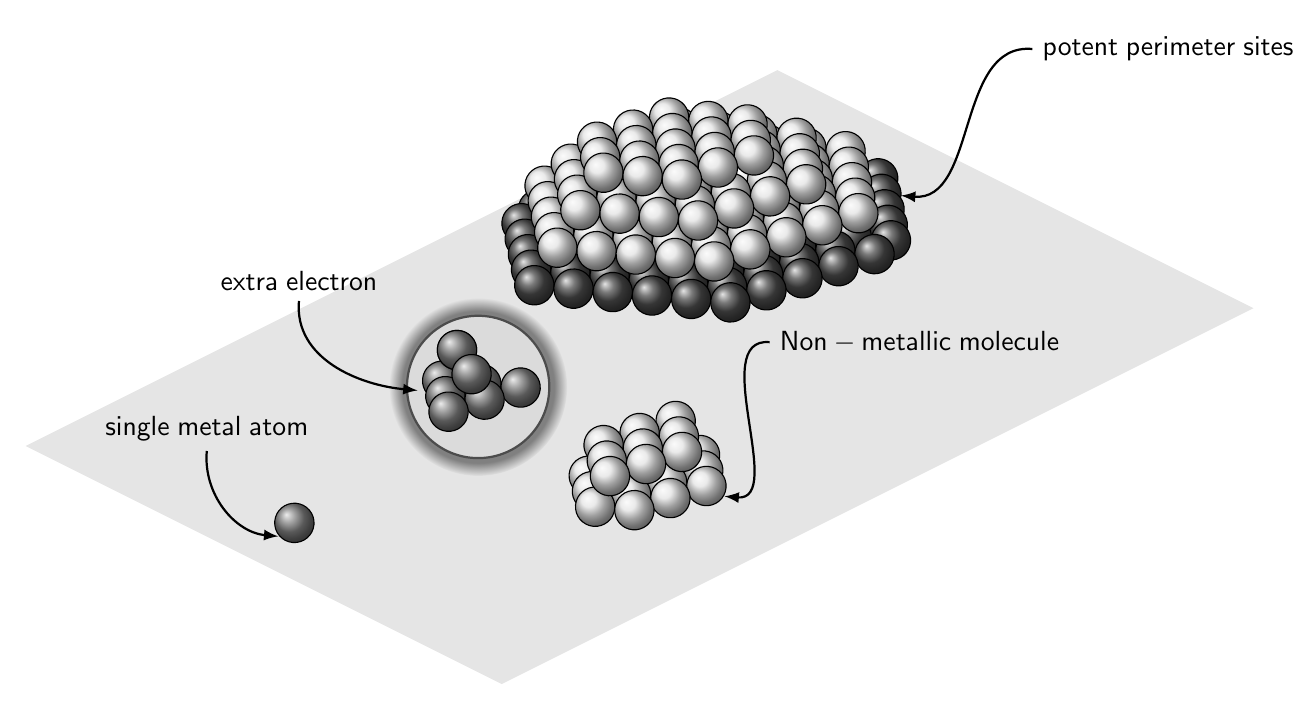
\begin{tikzpicture}
%\draw[help lines] (0,0) grid (10,10); %used just for visualising the positions of objects during construction

\begin{scope}[yshift=-180,yslant=0.5,xslant=-1]
    %the rectangular surface onto which the clusters are located
    \filldraw[black!10,very thick] (0.5,1) rectangle (10,7);
    %circle circumventing the smallest cluster 
    \node[circle,circular glow,fill=red!20,draw=red,thick]
    at (4.1,4.9) {\phantom{perimetro}};
\end{scope}

%atom clusters are rotated for a better visualisation
\begin{scope}[rotate around = {-5:(0,0,0)}]
    %text describing the objects in the picture
    \draw[-latex,thick] (6,3) node[right,text width=3cm] 
        {$\mathsf{potent\; perimeter\; sites}$} to [out=180,in=0] (4.5,1);
    \draw[-latex,thick](3,-1)node[right]
        {$\mathsf{Non-metallic\; molecule}$} to[out=180,in=0] (2.6,-3);
    \draw[-latex,thick](-3,-1)node[above]
        {$\mathsf{extra \; electron}$} to[out=-90,in=180] (-1.4,-2);

    %now we start with the clusters (maybe this code could be improved by a tikz expert)
    %the layers are built starting from the very lowest one

    %largest cluster
    %first row
    \foreach \x  in {1.5,2,2.5,3,3.5,4}%
        \shadedraw [ball color= red] (\x,1,-0.5) circle (0.25cm);
    \foreach \x  in {1.25,1.75,2.25,2.75,3.25,3.75,4.25}%
        \shadedraw [ball color= red] (\x,1,0) circle (0.25cm);
    \foreach \x  in {1,1.5,2,2.5,3,3.5,4,4.5}%
        \shadedraw [ball color= red] (\x,1,0.5) circle (0.25cm);
    \foreach \x  in {0.75,1.25,1.75,2.25,2.75,3.25,3.75,4.25,4.75}%
        \shadedraw [ball color= red] (\x,1,1) circle (0.25cm);
    \foreach \x  in {0.5,1,1.5,2,2.5,3,3.5,4,4.5,5}%
        \shadedraw [ball color= red] (\x,1,1.5) circle (0.25cm);
    \foreach \x  in {0.5,1,1.5,2,2.5,3,3.5,4,4.5,5}
        \shadedraw [ball color=red] (\x,1,2) circle (0.25cm);
    \foreach \x  in {0.75,1.25,1.75,2.25,2.75,3.25,3.75,4.25,4.75}%
        \shadedraw [ball color= red] (\x,1,2.5) circle (0.25cm);
    \foreach \x  in {1,1.5,2,2.5,3,3.5,4,4.5}%
        \shadedraw [ball color= red] (\x,1,3) circle (0.25cm);
    \foreach \x  in {1.25,1.75,2.25,2.75,3.25,3.75,4.25}%
        \shadedraw [ball color= red] (\x,1,3.5) circle (0.25cm);
    \foreach \x  in {1.5,2,2.5,3,3.5,4}%
        \shadedraw [ball color= red] (\x,1,4) circle (0.25cm);
    %second row 
    \foreach \x  in {1.75,2.25,2.75,3.25,3.75}
        \shadedraw [ball color=yellow] (\x,1.5,0) circle (0.25cm);
    \foreach \x  in {1.5,2,2.5,3,3.5,4}
        \shadedraw [ball color=yellow] (\x,1.5,0.5) circle (0.25cm);
    \foreach \x  in {1.25,1.75,2.25,2.75,3.25,3.75,4.25}
        \shadedraw [ball color=yellow] (\x,1.5,1) circle (0.25cm);
    \foreach \x  in {1,1.5,2,2.5,3,3.5,4,4.5}
        \shadedraw [ball color=yellow] (\x,1.5,1.5) circle (0.25cm);
    \foreach \x  in {0.75,1.25,1.75,2.25,2.75,3.25,3.75,4.25,4.75}
        \shadedraw [ball color=yellow] (\x,1.5,2) circle (0.25cm);
    \foreach \x  in {1,1.5,2,2.5,3,3.5,4,4.5}
        \shadedraw [ball color=yellow] (\x,1.5,2.5) circle (0.25cm);
    \foreach \x  in {1.25,1.75,2.25,2.75,3.25,3.75,4.25}
        \shadedraw [ball color=yellow] (\x,1.5,3) circle (0.25cm);
    \foreach \x  in {1.5,2,2.5,3,3.5,4}
        \shadedraw [ball color=yellow] (\x,1.5,3.5) circle (0.25cm);
    \foreach \x  in {1.75,2.25,2.75,3.25,3.75}
        \shadedraw [ball color=yellow] (\x,1.5,4) circle (0.25cm);
    %third row 
    \foreach \x  in {2,2.5,3,3.5}
        \shadedraw [ball color=yellow] (\x,2,1) circle (0.25cm);
    \foreach \x  in {1.75,2.25,2.75,3.25,3.75}
        \shadedraw [ball color=yellow] (\x,2,1.5) circle (0.25cm);
    \foreach \x  in {1.5,2,2.5,3,3.5,4}
        \shadedraw [ball color=yellow] (\x,2,2) circle (0.25cm);
    \foreach \x  in {1.25,1.75,2.25,2.75,3.5,3.75,4.25}
        \shadedraw [ball color=yellow] (\x,2,2.5) circle (0.25cm);
    \foreach \x  in {1.5,2,2.5,3,3.5,4}
        \shadedraw [ball color=yellow] (\x,2,3) circle (0.25cm);
    \foreach \x  in {1.75,2.25,2.75,3.25,3.75}
        \shadedraw [ball color=yellow] (\x,2,3.5) circle (0.25cm);
    \foreach \x  in {2,2.5,3,3.5}
        \shadedraw [ball color=yellow] (\x,2,4) circle (0.25cm);
    %fourth row
    \foreach \x  in {2.25,2.75,3.25}
        \shadedraw [ball color=yellow] (\x,2.5,2) circle (0.25cm);
    \foreach \x  in {2,2.5,3,3.5}
        \shadedraw [ball color=yellow] (\x,2.5,2.5) circle (0.25cm);
    \foreach \x  in {1.75,2.25,2.75,3.25,3.75}
        \shadedraw [ball color=yellow] (\x,2.5,3) circle (0.25cm);
    \foreach \x  in {2,2.5,3,3.5}
        \shadedraw [ball color=yellow] (\x,2.5,3.5) circle (0.25cm);
    \foreach \x  in {2.25,2.75,3.25}
        \shadedraw [ball color=yellow] (\x,2.5,4) circle (0.25cm);

    %medium cluster
    %first row
    \foreach \x  in {6.75,7.25}
        \shadedraw [ball color=yellow] (\x,2.5,13) circle (0.25cm);
    \foreach \x  in {6.5,7,7.5}
        \shadedraw [ball color=yellow] (\x,2.5,13.5) circle (0.25cm);
    \foreach \x  in {6.25,6.75,7.25,7.75}
        \shadedraw [ball color=yellow] (\x,2.5,14) circle (0.25cm);
    \foreach \x  in {6.5,7,7.5}
        \shadedraw [ball color=yellow] (\x,2.5,14.5) circle (0.25cm);
    \foreach \x  in {6.75,7.25}
        \shadedraw [ball color=yellow] (\x,2.5,15) circle (0.25);

    %second row
    \foreach \x  in {7} %this foreach is used to be general, but it makes no sense if we put just one sphere!
        \shadedraw [ball color=yellow] (\x,3,13.25) circle (0.25cm);
    \foreach \x  in {6.75,7.25}
        \shadedraw [ball color=yellow] (\x,3,13.75) circle (0.25cm);
    \foreach \x  in {6.5,7,7.5}
        \shadedraw [ball color=yellow] (\x,3,14.25) circle (0.25cm);
    \foreach \x  in {6.75,7.25}
        \shadedraw [ball color=yellow] (\x,3,14.75) circle (0.25cm);
    \foreach \x  in {7}
        \shadedraw [ball color=yellow] (\x,3,15.25) circle (0.25);

    %smallest cluster of atoms

    \foreach \x in {2.75,3.25,3.75}
        \shadedraw [ball color = gray] (\x,2,10) circle (0.25);
    \foreach \x in {3,3.5}
        \shadedraw [ball color=gray] (\x,2,10.5) circle (0.25);
    \shadedraw [ball color = gray] (3.25,2,11) circle (0.25);
    \foreach \x in {3,3.5}
        \shadedraw [ball color = gray] (3,2.5,10.25) circle (0.25);
    \shadedraw [ball color = gray] (3.5,2.5,11) circle (0.25);

    \shadedraw [ball color=gray] (2,1,12.5) circle(0.25);
    \draw[-latex,thick](-4,-3)node[above]
        {$\mathsf{single \; metal\; atom}$} to[out=-90,in=180] (-3,-4);
\end{scope}
\end{tikzpicture}
\end{document} 